\section{Overview: High-level components and their interaction}
	Our system will be developed as a 4-tiered JEE application, divided as Client Tier, Web Tier, Business Tier and the EIS Tier. It is distributed between client machines, Java EE server machine and the database.
	\\The diagram below provides a better understanding of the components of our system, highlighting the interactions among them:
	%\subsubsection{Architecture Component Diagram}
	\begin{figure}[!ht]
	  \centering
	  \vspace{0.2cm}
	  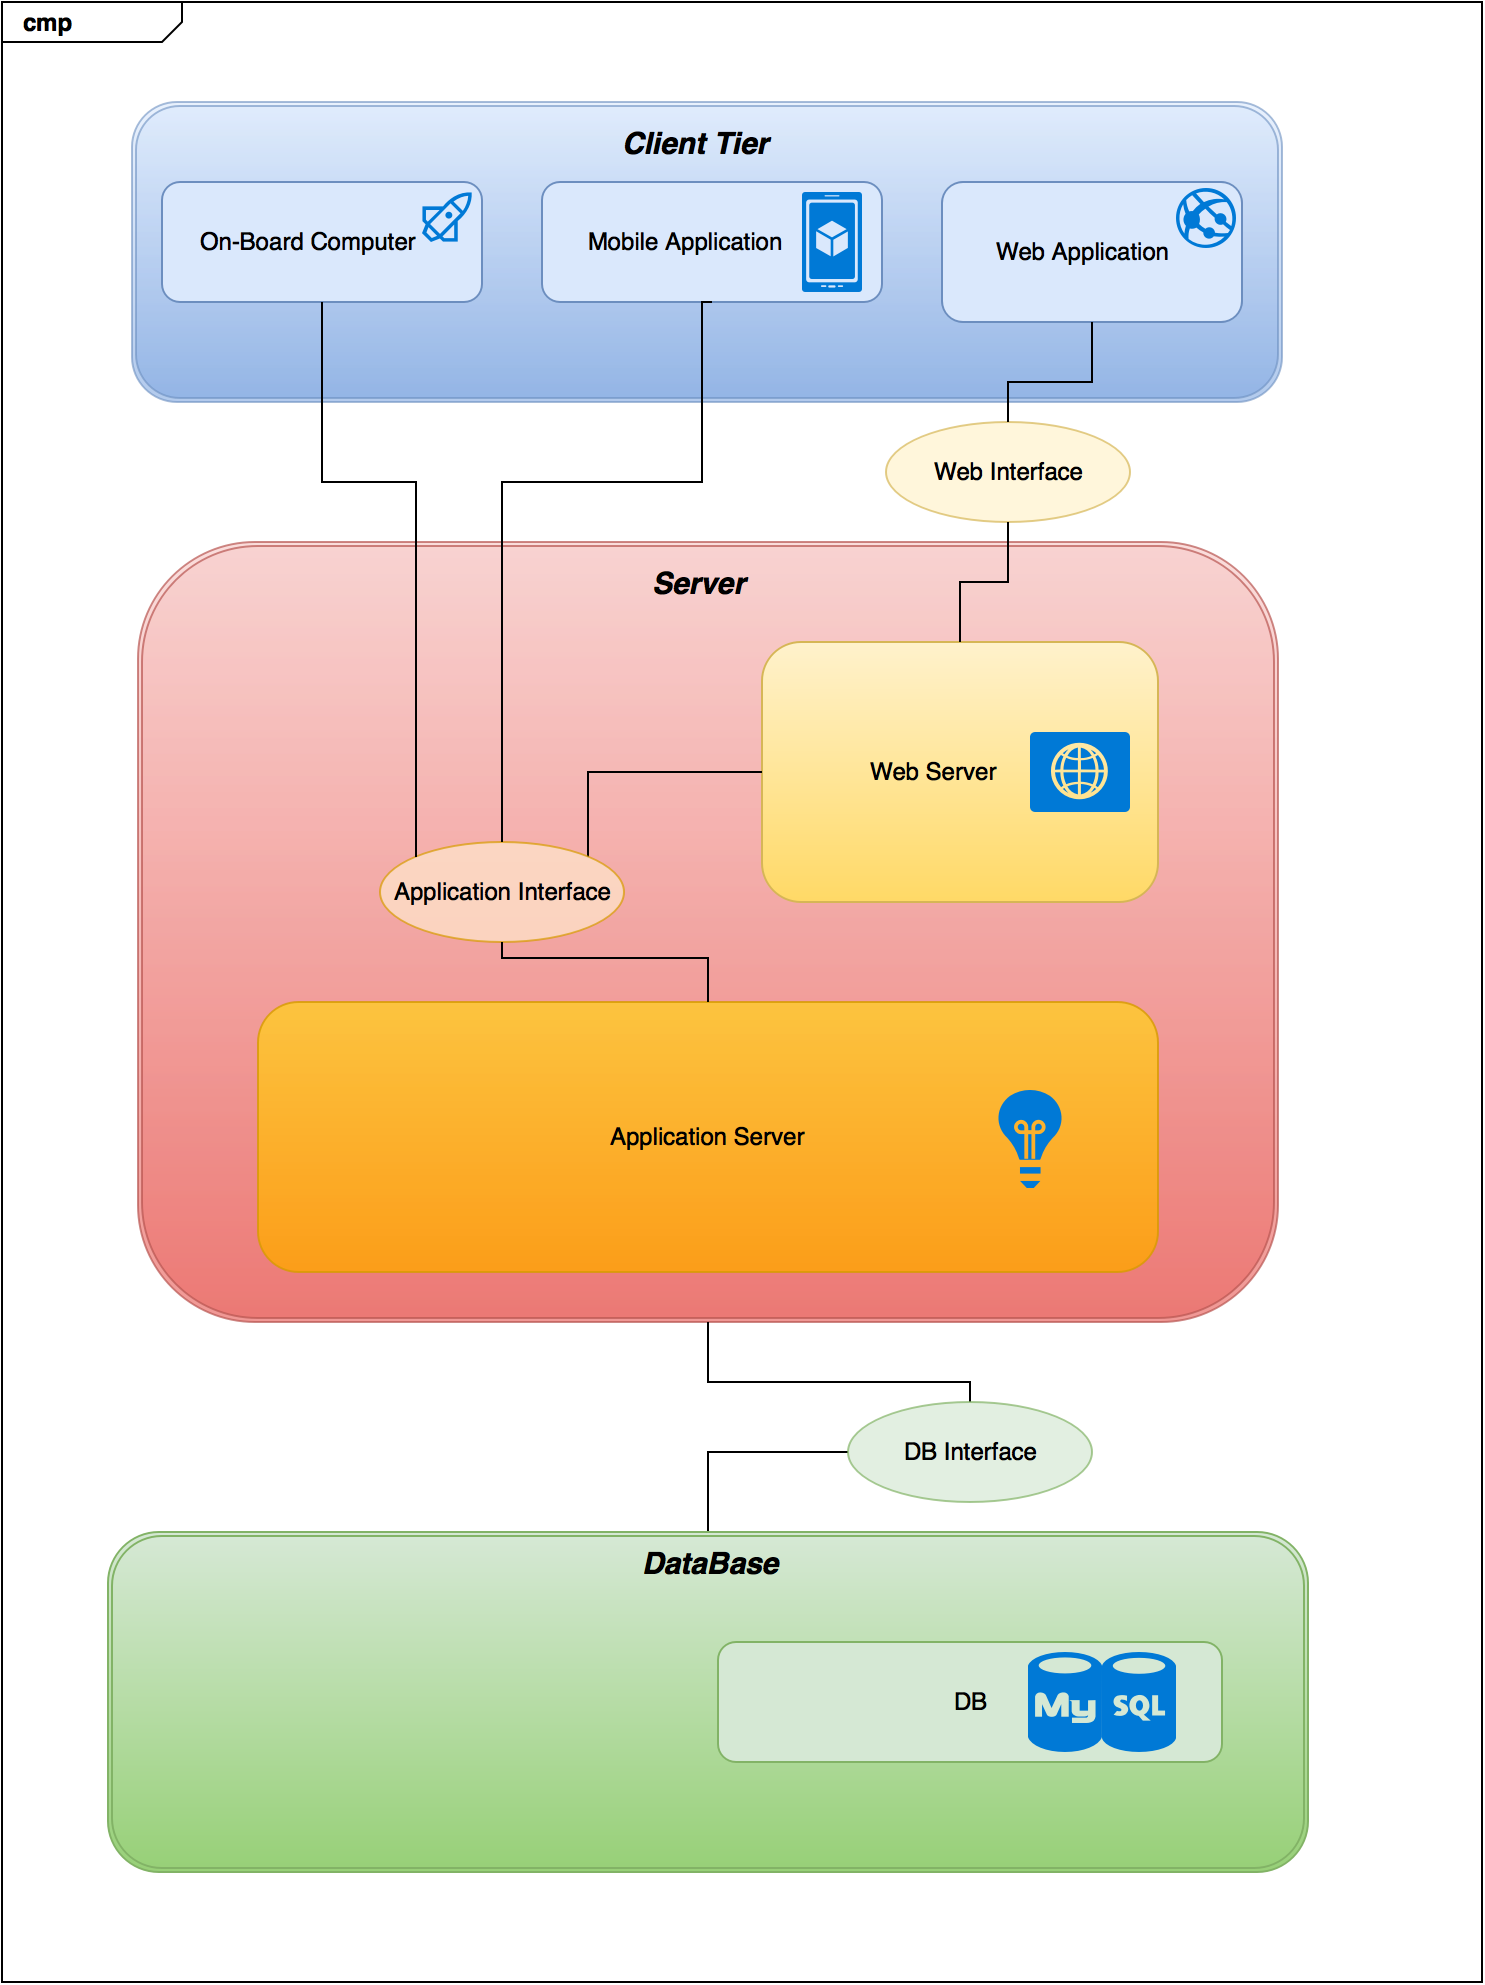
\includegraphics[width=0.6\textwidth]{/DD/4-Tier_Architecture}\\
	  \vspace{0.4cm}
	  %\caption{PowerEnJoy architecture} 
	  \label{fig:4-Tier_Architecture} 
	\end{figure}
\section{Component view}
	\blindtext
\section{Deployment view}
	\blindtext
\section{Runtime view}
	\blindtext
\section{Component Interfaces}
	\blindtext
\section{Selected architectural styles and patterns}
	\blindtext
\section{Other design decisions}
	\blindtext